\documentclass[reprint,english,notitlepage]{revtex4-2}  % defines the basic parameters of the document

\usepackage[utf8]{inputenc}
\usepackage[english]{babel}

\usepackage{physics,amssymb}  % mathematical symbols (physics imports amsmath)
\usepackage{graphicx}         % include graphics such as plots
\usepackage{xcolor}           % set colors
\usepackage{hyperref}         % automagic cross-referencing (this is GODLIKE)
\usepackage{tikz}             % draw figures manually
\usepackage{listings}         % display code
\usepackage{subfigure}        % imports a lot of cool and useful figure commands

\hypersetup{ % this is just my personal choice, feel free to change things
    colorlinks,
    linkcolor={red!50!black},
    citecolor={blue!50!black},
    urlcolor={blue!80!black}}

\lstset{ %
	inputpath=,
	backgroundcolor=\color{white!88!black},
	basicstyle={\ttfamily\scriptsize},
	commentstyle=\color{magenta},
	language=Python,
	morekeywords={True,False},
	tabsize=4,
	stringstyle=\color{green!55!black},
	frame=single,
	keywordstyle=\color{blue},
	showstringspaces=false,
	columns=fullflexible,
	keepspaces=true}



\begin{document}
\title{Analysis of APEX CO(2-1) emission line observation of a nearby galaxy}   % self-explanatory
\author{Rebecca Nguyen}               % self-explanatory
\date{\today}                             % self-explanatory
\noaffiliation                            % ignore this
\begin{abstract}                          % marks the beginning of the abstract
This abstract is abstract.                % the body of the abstract
\end{abstract}                            % marks the end of the abstract
\maketitle                                % creates the title, author, date & abstract


% the fundamental components of scientific reports:
\section{Introduction}
% Your goal is to analyze the CO(2-1) line emission of the galaxy IRAS 13120-5453.

\section{Theory}   % (optional)
% Single-dish
\subsection{Single-dish}
The primary mirror is the first optical element of a telescope, encountered by light. The telescope's primary mirror is called a dish in radio/(sub-) mm bands (bands meaning frequency observation windows). Radio/(sub-)mm telescopes are either made with 1) A single dish meaning one single antenna connected to one or several receivers 2) $N\geq$ 2 antennas working as an interferometer. The second option provides a larger collecting area and better spatial resolution. However, single dishes are very optimal for studying very extended, low surface brightness structures and/or for surveys of large areas of the sky \cite{lecturenotes}.

Examples of radio and sub-millimeter single-dish facilities are APEX and LMT. Atacama Pathfinder Experiment, APEX, operates at millimeter and submillimetre wavelengths - between infrared light and radio waves. It is placed at an elevation of 5100 meters in Chile's Atacama region \cite{APEX website}.
The Large Millimeter Telescope is situated in Volcán Sierra Negra at an altitude of 4600 meters and is specifically designed to observe in the wavelength range of 0.85 - 4 mm \cite{LMT website}.

\begin{figure}[h!]
    \centering
    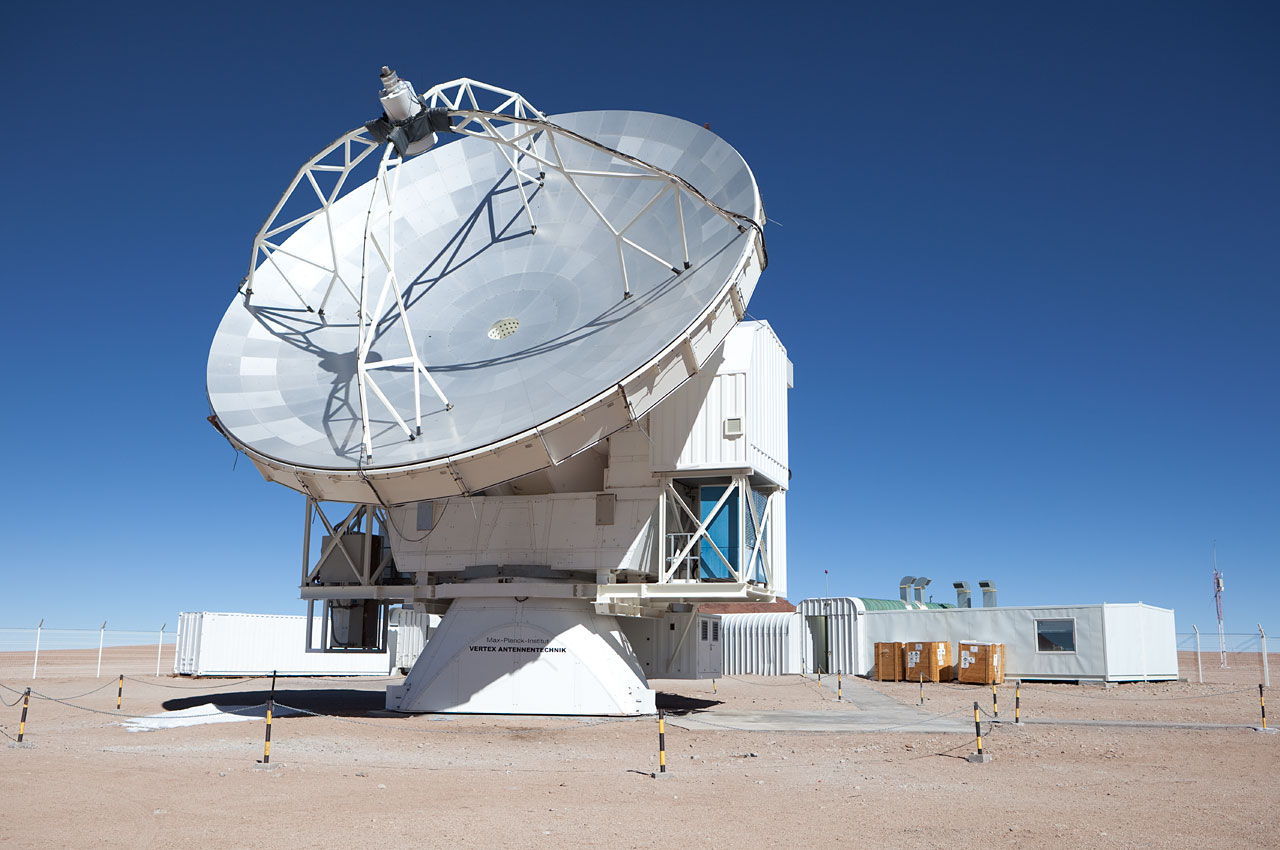
\includegraphics[scale = 0.13]{apex-mar2009-1671.jpeg} \hfill
    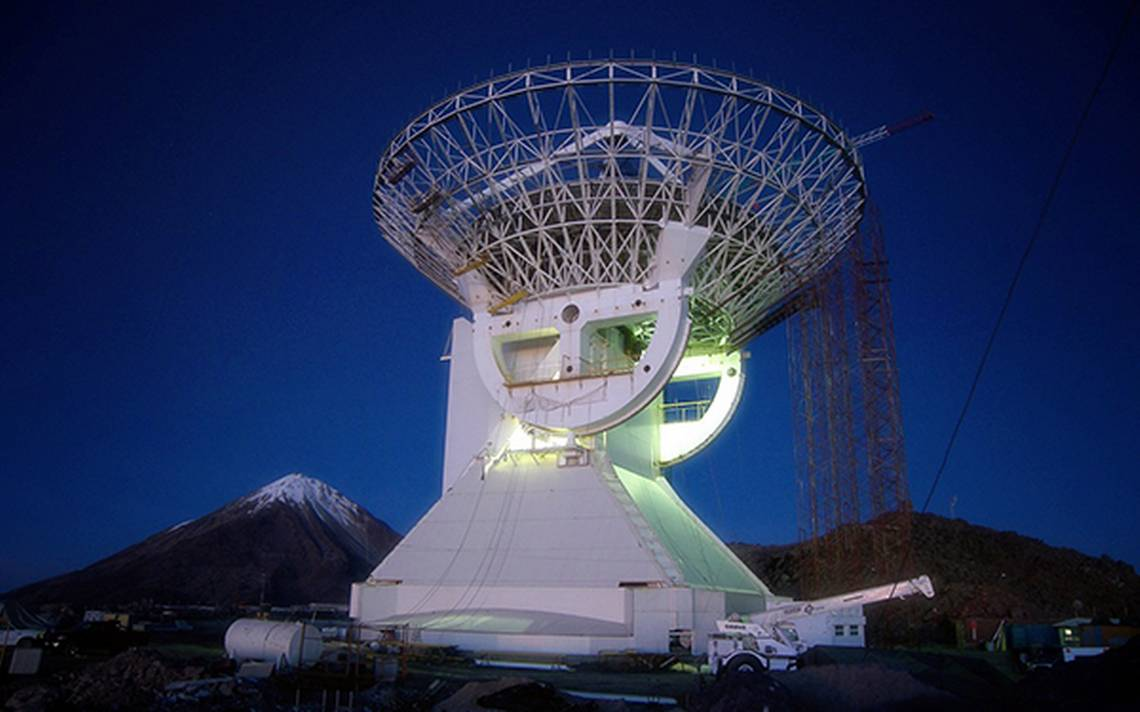
\includegraphics[scale = 0.146]{galGTM16.jpeg}
    \caption{APEX depicted in the image on top \cite{APEX image} and LMT depicted on the bottom \cite{LMT image}.}
\end{figure}

% Antenna temperature
The antenna temperature is equal to the brightness temperature of the source convolved with the normalized beam pattern of the antenna \cite{lecturenotes}.
\begin{equation} \label{eq: K/Jy}
    F_\nu \equiv \Gamma F_\nu \rightarrow F_\nu = \Gamma^{-1}F^*_A
\end{equation}



\begin{equation} \label{eq: luminosity}
    L_{CO}^{'}[K\textbf{ }km/s pc^2] = (3.25 \cdot 10^7)\frac{D_L^2}{V_{obs^2}(1 + z)^3} \int_{\Delta \nu}S_\nu d\nu
\end{equation}

\begin{equation} \label{total molecular gas mass}
    M_{H_2 + He}[M_{\odot}]= \alpha_{CO}L_{CO}^{'}
\end{equation}

\section{Method}
% Class
The data obtained from APEX consist of observations from different sources, among other things, the observation of
the molecular line transition CO(2-1) of the galaxy IRAS 13120-5453, a nearby ultraluminous infrared galaxy. The redshift of this galaxy is $z = 0.0308$, which corresponds to a luminosity distance of $D_L = 139.4 Mpc$ (using $H_0 = 67.8 km/s$, $\Omega_M = 0.307$, $\Omega_\Lambda = 0.693$ and $k = 0$, i.e. flat geometry) \cite{task description}.

\subsection{Curve fit by Gaussian profile}

Our goal is to analyze the CO(2-1) emission line. As emission lines closely resemble a Gaussian curve, it is, therefore, an interest to curve fit a Gaussian profile to the emission line.
\begin{equation} \label{gaussian}
    g(x, \mathbf{P})=ae^{-\frac{(x - b)^2}{2c^2}} + d; \textbf{ P} = (a, b, c, d)
    \label{eq: gauss}
\end{equation}

The purpose of the fitting is to optimize the parameters in P based on the data. The parameters are as follows

\indent a: the amplitude of the Gaussian. The difference in the minimum value of your spectral line and the minimum.\\
\indent b: the mean of the gaussian. The position of the peak on the x-axis.\\
\indent c: width of the Gaussian.\\
\indent d. y-value of the baseline. The maximum value of the spectrum \\

\section{Results}
\begin{figure}[h!]
    \centering
    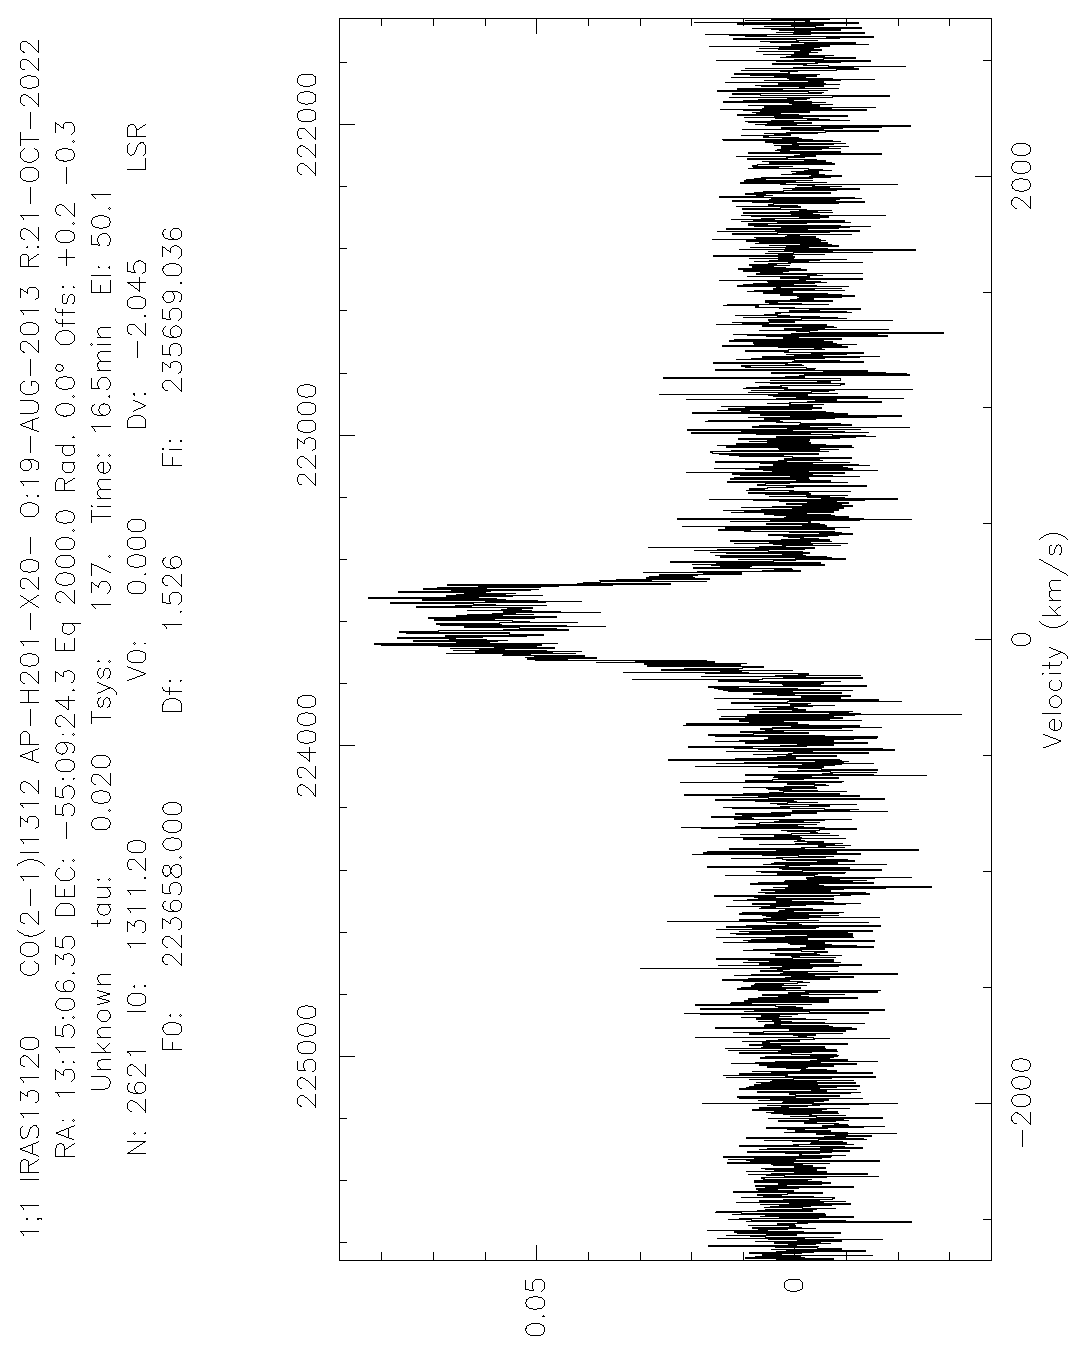
\includegraphics[scale = 0.4, angle = -90]{spect_only.eps}
    \caption{Caption}
    \label{fig: reduced data class}
\end{figure}

\section{Discussion}
\section{Conclusion}
% acknowledgments (optional)
\begin{acknowledgments}  % if you disagree with the spelling, blame Americans
I would like to thank myself for writing this beautiful document.
\end{acknowledgments}


\newpage

\appendix
\section{Name of appendix}
This will be the body of the appendix.
\section{This is another appendix}\label{appendix}
Tada.



\clearpage
\onecolumngrid
\section{References}
\begin{thebibliography}{9}

\bibitem{lecturenotes}
Cicone, C. (2022, October 21). AST2210 Lecture 6: Sub-millimeter/radio observations (single-dish). \href{https://bibsys-k.alma.exlibrisgroup.com/leganto/public/47BIBSYS_UBO/citation/14898320160002204?auth=SAML}{[PDF]}.

\bibitem{APEX website}
(-). APEX Reaching new heights in submillimetre astronomy. ESO.[Website]. \href{https://www.eso.org/public/teles-instr/apex/}{[website]}

\bibitem{LMT website}
(-). Large Millimeter Telescope. Large Millimeter Telescope. \href{http://lmtgtm.org/}{[Website]}

\bibitem{APEX image}
(2009). APEX antenna [Photograph]. \href{https://www.eso.org/public/images/apex-mar2009-1671/}{[Photograph]}

\bibitem{LMT image}
(-). Large Millimiter Telescope or LMT. \href{https://mxcity.mx/wp-content/uploads/2019/04/galGTM16.jpeg}{[Photograph]}

\bibitem{task description}
Arroyave, I. M. (2022, October 21). Analysis of APEX CO(2-1) emission line observation of a nearby galaxy. \href{https://drive.google.com/file/d/1Y9YKh_9BOnJ547KBhBBsiDhk9iVBG3N6/view?usp=sharing}{[PDF]}.

\end{thebibliography}

\end{document}
